\chapter{Συστήματα Peer-to-Peer}
\label{chap:P2P}

\section{Εισαγωγή}
\ \ \ \ TODO

\section{Το P-Grid Σύστημα}

Το P-Grid 
\citep{Abererb, Aberer, Abererc, Abererd, Aberer2004, Aberer2003, Aberere, Aberer2002} 
είναι ένα πλήρως αποκεντρωμένο και δομημένο 
(structured) peer-to-peer σύστημα. Χρησιμοποιεί τυχαιοκρατικούς 
αλγορίθμους για την κατασκευή και την λειτουργία του. Η τοπολογία που 
δημιουργείται είναι ένα δυαδικό trie δέντρο και χρησιμοποιούνται 
προθέματα κλειδιών για την δρομολόγηση των μηνυμάτων μέσα στο δίκτυο.

Οι peer αποφασίζουν κατά ζεύγη τον τρόπο με τον οποίο θα 
χωρίσουν τον χώρο κλειδιών (key space). Κάθε κατάτμηση του χώρου 
αντιστοιχεί σε μια συγκεκριμένη δυαδική συμβολοσειρά ή οποία αποτελεί 
και το μονοπάτι ενός peer. Στο σχήμα \ref{fig:PGrid_overlay} φαίνεται η τελική 
διαμόρφωση του χώρου κλειδιών και της τοπολογίας που έχουν σχηματίσει οι 
peer. Το δίκτυο αποτελείται από τέσσερις peer κάθε ένας εκ των οποίων 
έχει συσχετιστεί με ένα μονοπάτι. Η ρίζα του δέντρου αποτελεί τον 
συνολικό χώρο των κλειδιών. Οι διακλαδώσεις σε κάθε ύψος αναπαριστούν 
κατατμήσεις του χώρου ένα ψηφίο τη φορά. Παράδειγμα, μετά την ρίζα, 
έχουν δημιουργηθεί δύο μεγάλα υπόδεντρα. Το αριστερό περιλαμβάνει όλα τα 
κλειδιά τα οποία έχουν πρόθεμα το \textit{'0'}, ενώ το αριστερό αυτά που έχουν 
πρόθεμα το \textit{'1'}. Συνεπώς, οι peer ανάλογα με το μονοπάτι με το οποίο 
έχουν συσχετιστεί, γνωρίζουν ένα συγκεκριμένο πλήθος κλειδιών.

\begin{figure}[h]
\centering
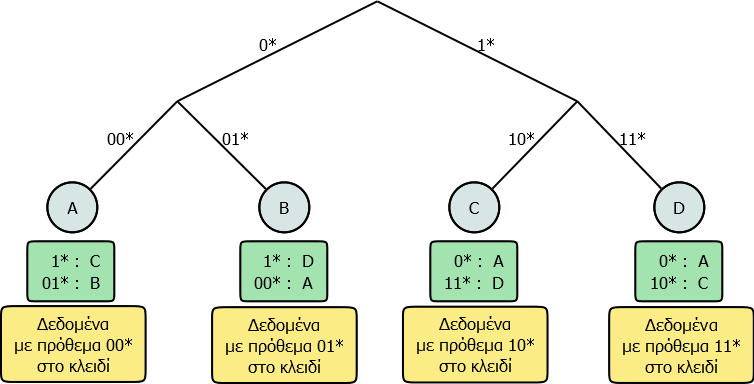
\includegraphics[scale=0.4]{Figures/P2P_PGrid/PGrid_overlay_network.png}
\caption{Η τοπολογία ενός δικτύου P-Grid}
\label{fig:PGrid_overlay}
\end{figure}

Για κάθε επίπεδο του δέντρου, αποθηκεύονται αναφορές στον πίνακα 
δρομολόγησης προς τους peer των οποίων το μονοπάτι ανήκει στο συζυγές 
υπόδεντρο. Παράδειγμα, ο peer Α έχει μονοπάτι \textit{'00'} και επομένως θα 
αποθηκεύσει αναφορές για το επίπεδο με μονοπάτι \textit{'0'} έναν peer από το 
συζυγές του που είναι το υπόδεντρο με μονοπάτι \textit{'1'}. Αντίστοιχα για το 
\textit{'00'} είναι το \textit{'01'}. Στο σχήμα \ref{fig:PGrid_overlay} έχει 
συσχετίσει το \textit{'1'} με τον peer C και το \textit{'01'} με τον B. 
Η επιλογή των peer που θα επιλέξει να κρατήσει αναφορές είναι τυχαία. Επίσης, 
οι peer που αποθηκεύονται ανά επίπεδο μπορεί είναι να περισσότεροι του ενός. 
Βάσει αυτής της τοπολογίας, μια αναζήτηση θα κάνει Ο(logN) βήματα μέχρι να 
βρεθεί το αποτέλεσμα της. Άλλο πλεονέκτημα είναι και η δυνατότητα εκτέλεσης 
αναζητήσεων με δεδομένο ένα εύρος κλειδιών (key range).

Όσον αφορά τα δεδομένα που μπορεί να αποθηκεύσει κάθε peer, 
ακολουθείται η ίδια λογική. Υπάρχει μια συνάρτηση κατακερματισμού η 
οποία αντιστοιχεί κλειδιά σε δεδομένα. Κάθε peer είναι υπεύθυνος για 
εκείνο το κομμάτι των δεδομένων που έχει πρόθεμα το μονοπάτι του.

Τέλος, το σύστημα υποστηρίζει διάφορα πρωτόκολλα. Αυτό που μας 
ενδιαφέρει στην παρούσα εργασία είναι αυτό της ανοχής λαθών 
(fault-tolerance). Αυτό που προτείνεται και είναι και υλοποιημένο είναι 
η τεχνική της αντιγραφής (replication). Κάθε μονοπάτι του δέντρου 
αντιστοιχεί σε πολλαπλούς peer. Αυξάνει την γενική αντοχή του συστήματος 
σε αποτυχίες peer. Το κόστος είναι η μείωση της χωρητικότητας του 
δικτύου αφού μέρος των peer είναι αντίγραφα άλλων. Επίσης γίνεται πιο 
πολύπλοκη η διατήρηση και ο συγχρονισμός του συστήματος. 
